\subsection{Détection et diagnostic des défauts}
\label{sec:detection}

\paragraph{Objectif.} Un outil de détection doit remplir deux conditions. D'abord, il ne doit pas déclencher d'alarme quand tout va bien : des fausses alarmes répétées font perdre confiance à l'opérateur, qui finit par les ignorer~\cite{isa182}. Ensuite, quand un défaut survient, il doit le détecter et lui donner le bon nom. Nous avons vérifié ces deux conditions par deux tests, à l'aide du script \nolinkurl{ml/detection_defauts/evaluer_detection.py}.

\paragraph{Test 1 -- Fonctionnement normal.} Les dix règles sont appliquées à chacune des 43\,200 minutes du mois de juillet, exactement comme le fait le backend : médiane des 10 dernières minutes, puis hystérésis. Sur tout le mois, l'outil ne signale que \textbf{deux événements}, tous deux réels (tableau~\ref{tab:evtnormaux}, figure~\ref{fig:frise}).

\begin{table}[H]
\centering
\caption{Événements signalés sur le mois de fonctionnement normal (juillet 2026)}
\label{tab:evtnormaux}
\small
\begin{tabularx}{\textwidth}{>{\raggedright\arraybackslash}p{3.4cm} >{\raggedright\arraybackslash}p{4.6cm} X}
\toprule
\textbf{Défaut signalé} & \textbf{Période} & \textbf{Réalité} \\
\midrule
Usure des apex (cyclones) & Alerte le 16/07 à 06:04 (45\,\%), alarme le 18/07 à 06:45 (50\,\%), fin le 19/07 & Usure réelle : les apex ont été remplacés le 19/07 (ordres de travail WO-2026-0719). \\
Cyclone hors service & 17/07, de 16:48 à 19:45 & Un cyclone a réellement été arrêté de 16:44 à 19:40 : détection avec 4 minutes de retard. \\
\bottomrule
\end{tabularx}
\end{table}

\begin{figure}[H]
\centering
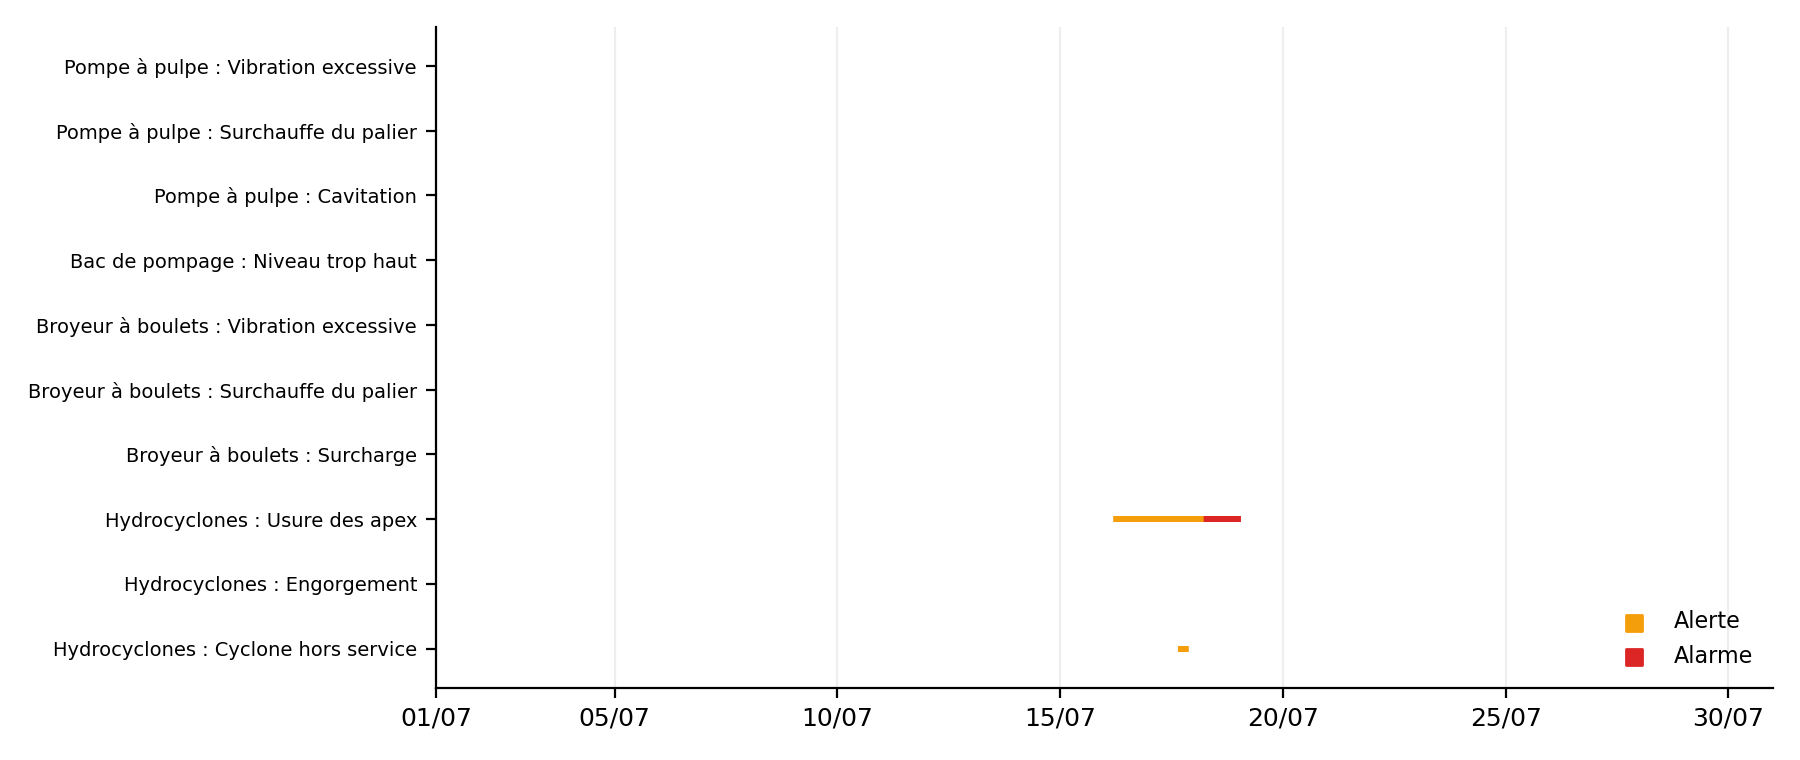
\includegraphics[width=\textwidth]{frise_defauts_juillet}
\caption{Défauts signalés sur le mois de juillet, règle par règle (orange : alerte, rouge : alarme)}
\label{fig:frise}
\end{figure}

L'outil n'a produit \textbf{aucune fausse alarme}. Ce résultat tient à deux précautions, dont l'effet est mesuré au tableau~\ref{tab:filtrage} sur la règle d'usure des apex. Cette mesure est bruitée : elle oscille d'environ $\pm 1$\,\% autour de sa tendance. Lorsqu'elle approche du seuil de 45\,\%, elle le franchit et le refranchit des dizaines de fois. Sans précaution, l'alerte « clignote » donc : elle apparaît et disparaît 139 fois. La médiane sur 10 minutes filtre le bruit et ramène ce nombre à 16. L'hystérésis élimine le reste : une fois active, l'alerte ne disparaît que si l'usure redescend de 3 points sous le seuil. Ce principe, appelé bande morte, est recommandé par la norme de gestion des alarmes ISA-18.2~\cite{isa182}.

\begin{table}[H]
\centering
\caption{Effet du filtrage sur la règle d'usure des apex}
\label{tab:filtrage}
\small
\begin{tabular}{lc}
\toprule
\textbf{Traitement appliqué à la mesure} & \textbf{Nombre d'alertes distinctes} \\
\midrule
Dernière mesure seule & 139 \\
Médiane des 10 dernières minutes & 16 \\
Médiane + hystérésis (bande morte de 3\,\%) & \textbf{1} \\
\bottomrule
\end{tabular}
\end{table}

\paragraph{Test 2 -- Défauts injectés.} Les données ne contenant qu'un seul vrai défaut, nous avons injecté chacun des neuf défauts du tableau~\ref{tab:scenarios} à 300 instants tirés au hasard dans le mois, soit 2\,700 essais. Un essai est réussi si l'outil détecte le défaut, lui donne le bon nom et n'annonce aucun autre défaut.

\begin{table}[H]
\centering
\caption{Défauts injectés et résultats (300 essais par défaut)}
\label{tab:scenarios}
\small
\begin{tabularx}{\textwidth}{>{\raggedright\arraybackslash}p{3.6cm} X c}
\toprule
\textbf{Défaut} & \textbf{Effet sur les mesures} & \textbf{Bon diagnostic} \\
\midrule
Balourd de la roue de pompe & Vibration de la pompe : $+2{,}6$~mm/s & 100\,\% \\
Cavitation de la pompe & Niveau du bac à 30\,\%, pression et courant de la pompe $\times 0{,}65$ & 100\,\% \\
Surchauffe du palier de pompe & Température du palier : $+22$~°C & 100\,\% \\
Niveau du bac trop haut & Niveau du bac à 88\,\% & 100\,\% \\
Surchauffe du palier du broyeur & Température du palier côté entraînement : $+22$~°C & 100\,\% \\
Surcharge du broyeur & Puissance et courant du moteur $\times 1{,}4$ & 100\,\% \\
Vibration du broyeur & Vibration du broyeur : $+4{,}5$~mm/s & 100\,\% \\
Apex de cyclone bouché & Pression d'entrée $+100$~kPa, perte de charge $+28$~kPa & 100\,\% \\
Cyclone hors service & 3 cyclones en service au lieu de 4 & 100\,\% \\
\bottomrule
\end{tabularx}
\end{table}

Les 2\,700 essais sont tous réussis. Surtout, l'outil ne confond jamais deux défauts. C'est le rôle des règles à plusieurs symptômes. Par exemple, la cavitation exige à la fois un niveau bas, une pression basse et un courant bas : une simple baisse de pression ne suffit pas à la déclencher, et un niveau bas seul non plus.

\paragraph{Analyse critique.} Ces résultats doivent être lus avec recul :
\begin{itemize}
  \item \textbf{Les défauts injectés sont francs.} Ils sont appliqués d'un coup et avec une amplitude nette, si bien qu'un taux de 100\,\% était attendu : ce test vérifie surtout que chaque règle est correctement écrite et qu'elle ne se confond pas avec les autres. Un défaut réel s'installe souvent progressivement. Il serait alors détecté plus tard, au moment où il franchit le seuil.
  \item \textbf{Certains seuils viennent de la plage observée.} Les seuils des vibrations proviennent de la norme ISO 10816-3~\cite{iso10816}, et ceux des apex et du palier du broyeur de la GMAO. Les autres ont été fixés au-dessus de la plage observée pendant un mois de fonctionnement normal. Ils devront être validés avec les ingénieurs du site.
  \item \textbf{Les règles ne reconnaissent que les défauts prévus.} Un défaut d'un type nouveau ne sera signalé que s'il fait sortir une mesure de sa plage. C'est le prix de la simplicité et de l'explicabilité de l'approche.
  \item \textbf{Un retard de quelques minutes.} La médiane sur 10 minutes retarde la détection d'environ 5 minutes. C'est acceptable pour l'usure ou l'échauffement, qui évoluent lentement. Les déclenchements de sécurité rapides restent du ressort de l'automate.
\end{itemize}
